\documentclass{../source/Experiment}

\major{信息工程}
\name{姚桂涛}
\title{利用中值滤波降低噪声}
\stuid{3190105597}
\college{信息与电子工程学院}
\date{\today}
\lab{}
\course{数字图像处理}
\instructor{李东晓}
\grades{}
\expname{利用中值滤波降低噪声}
\exptype{设计验证}
\partner{}
\begin{document}
    \makecover
    \section{实验任务}
        本次选择的是PROJECT-05-02题目。
        
        \bfseries{利用中值滤波降低噪声}

        \begin{enumerate}
            \item 编写一个程序实现$3 \times 3$的中值滤波。
            \item 下载Fig.5.7(a)图片,并对其添加椒盐噪声,$Pa = Pb = 0.2$。
            \item 对(2)中的图像实现中值滤波,并和课本中的Fig.5.10(b)比较,说明差异原因。
        \end{enumerate}
    \section{算法设计}
        \subsection{中值滤波}
        用预定义的像素邻域中的中值代替像素的值,即:
        $$\hat{f}(x,y) = \underset{(r,c) \in S_{xy}}{median}\{ g(r,c)\}
        $$ 

    \section{代码实现}
        本次实验编程语言选择的是Matlab。

        实现中值滤波的核心代码如下:

        \lstinputlisting[
            language  =   matlab
            ]{第二次/my_median.m}

        其中median3取出某个像素的$3 \times 3$邻域,然后通过reshape函数转换为列向量,通过median函数得到中值M。

        实验完整代码附录。
    \section{实验结果}
        实验测试图像使用如下图像:
        \begin{figure}[H]
            \centering
            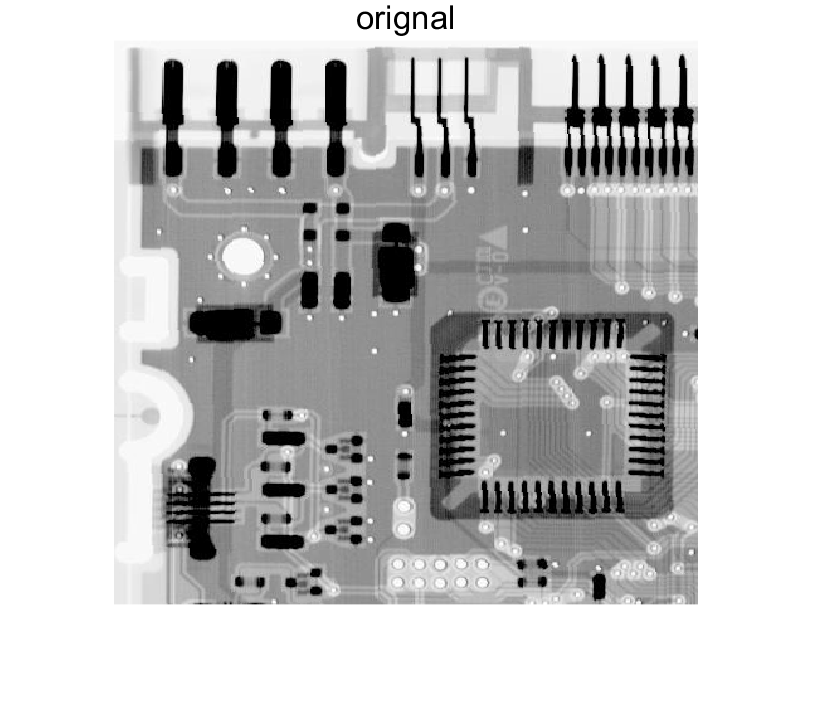
\includegraphics[width = 0.6\textwidth]{第二次/f1.png}
            \caption{测试图像}
        \end{figure}

        添加$Pa = Pb = 0.2$的椒盐噪声后如下:

        \begin{figure}[H]
            \centering
            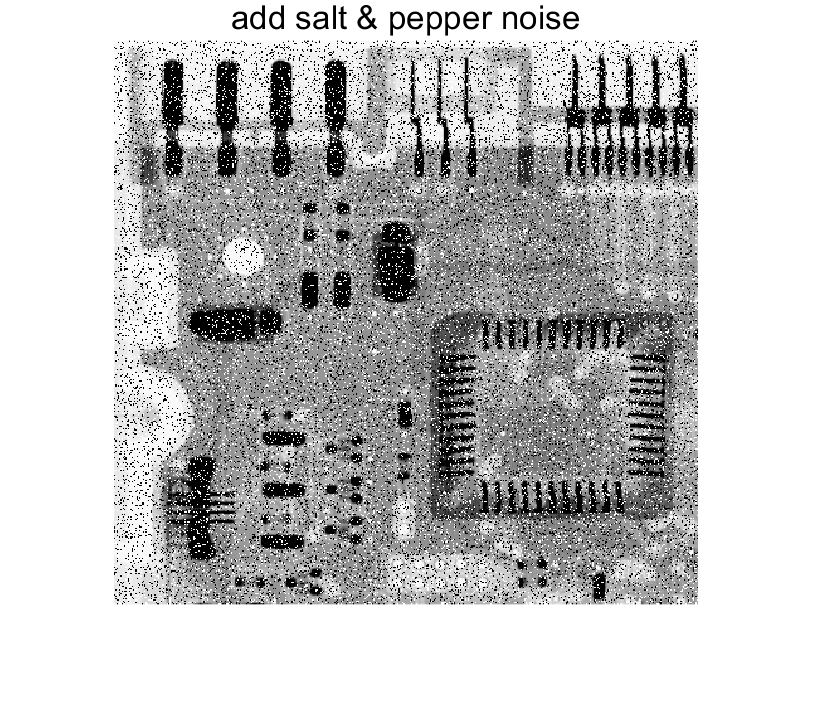
\includegraphics[width = 0.6\textwidth]{第二次/f2.png}
            \caption{添加椒盐噪声后}
        \end{figure}

        通过中值滤波后并与matlab自带的中值滤波图像对比:
        \begin{figure}[H]
            \centering
            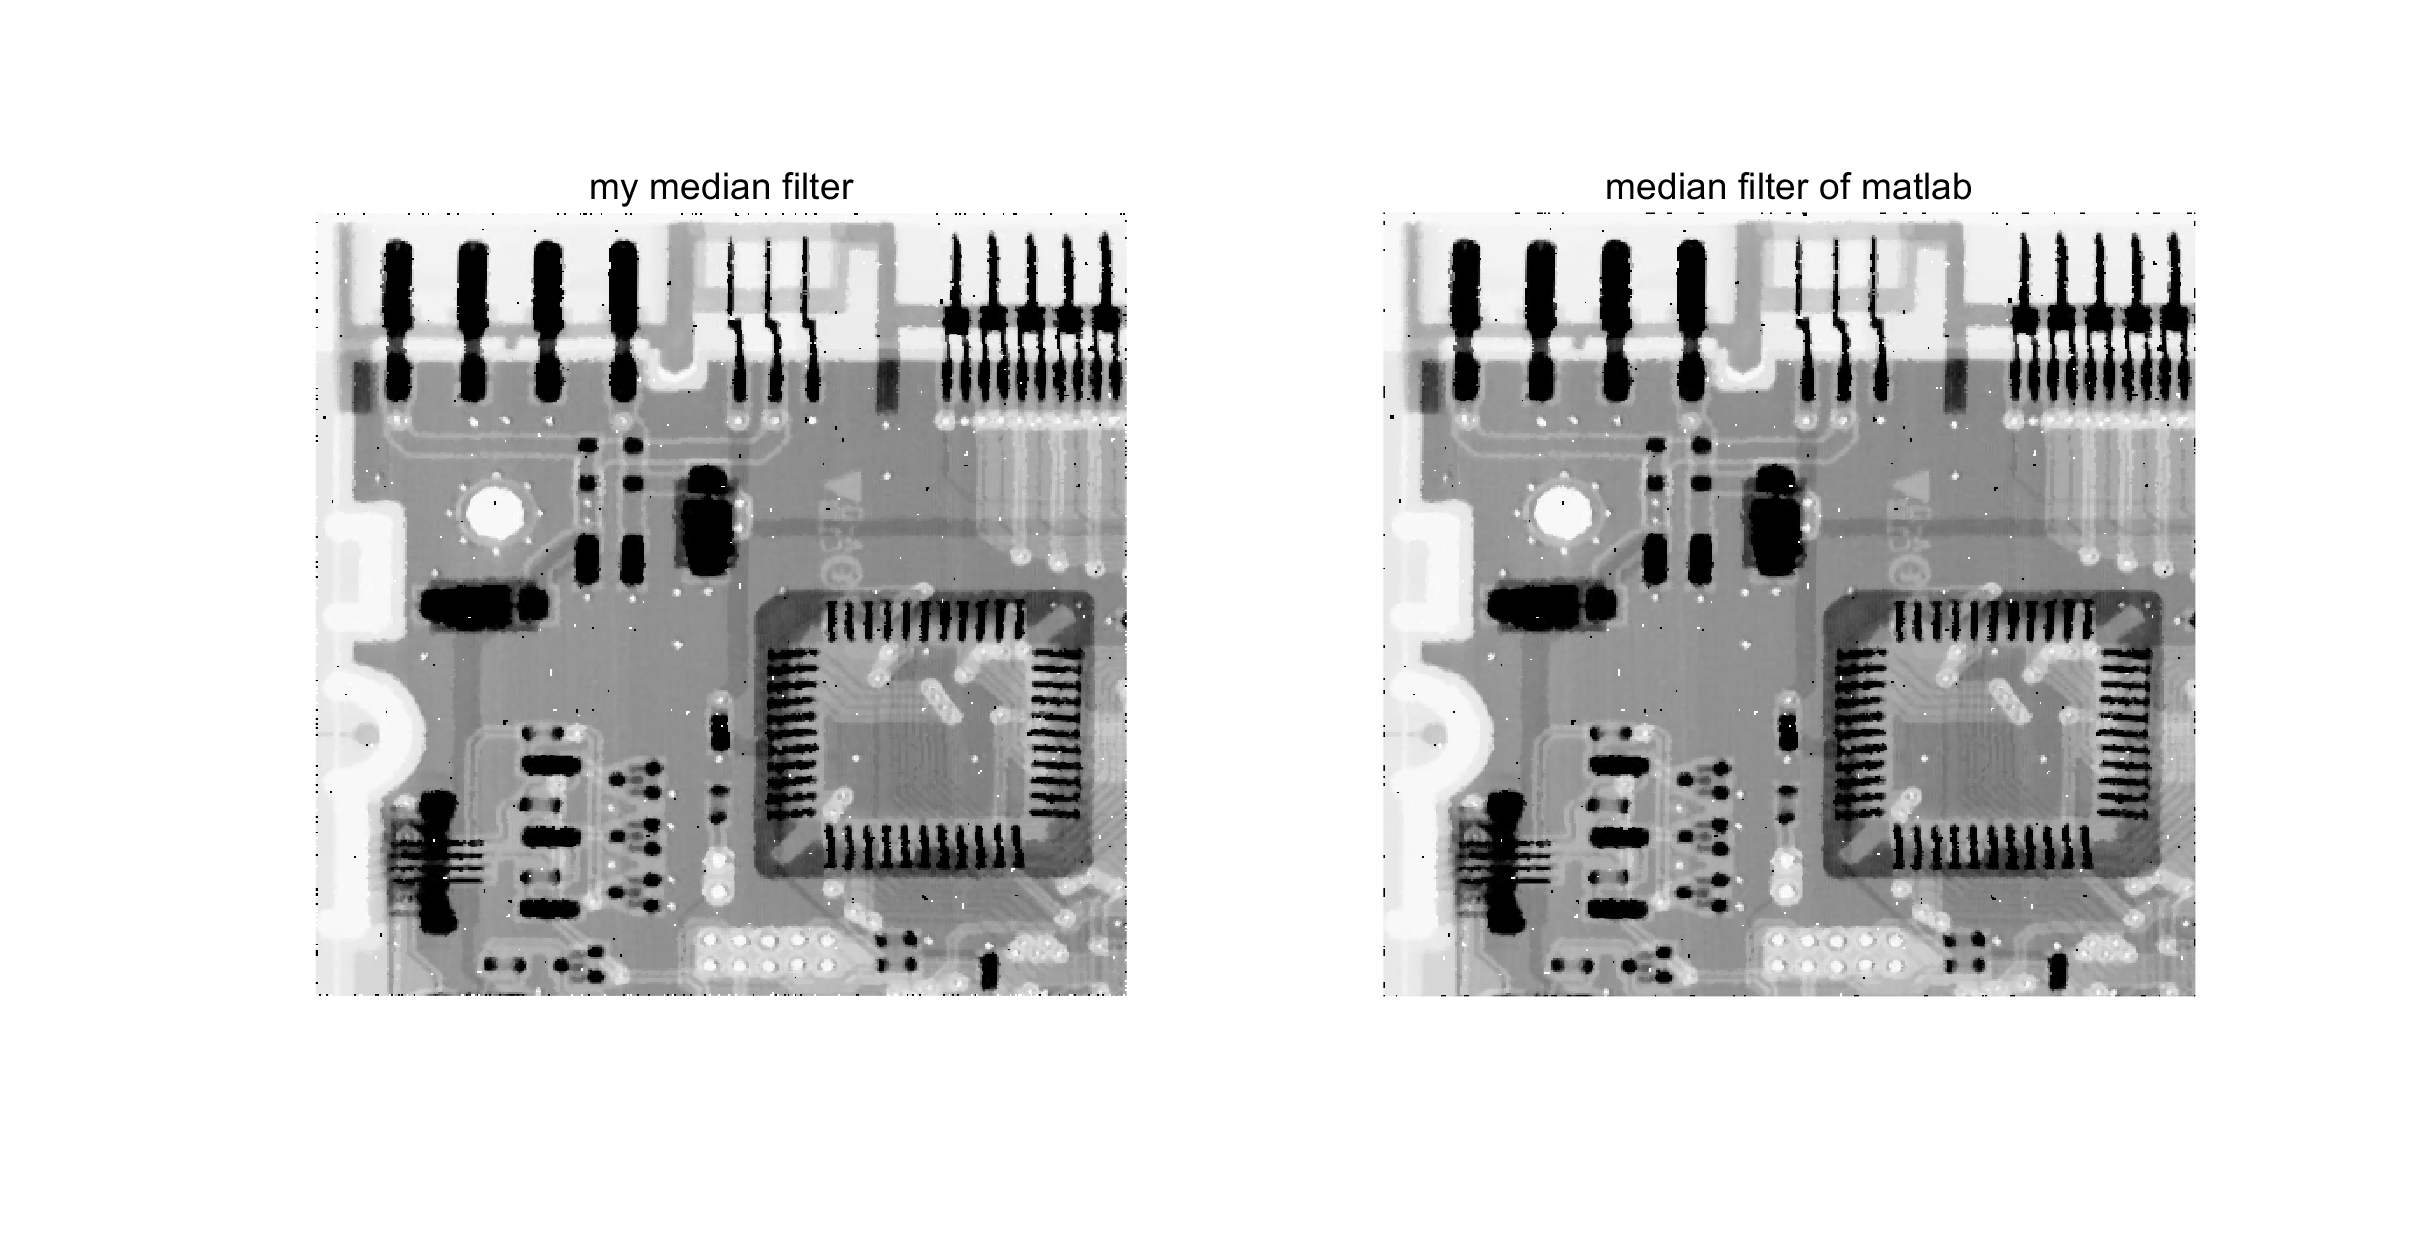
\includegraphics[width = 1\textwidth]{第二次/f3.png}
            \caption{中值滤波后}
        \end{figure}
        可以看到中值滤波后的大部分的椒盐噪声都被滤除,但还是有少量的噪声残留,同时与matlab自带的中值滤波函数对比,可以看到在图像边缘有些许不同,仍然有噪声存在,这是因为在实现滤波时,对于边缘的像素没有进行处理。

        改进措施应该对图像边缘进行边缘拓展。
    \section{总结}
    本次实验主要是通过Matlab编程语言实现了课程中所讲的中值滤波。
    
    在实验的过程中,我对于课程中所学的中值滤波理论有了更加深刻的理解,同时也意识到课程中所讲的内容与实际应用还有一定的差别,需要更多的理解与学习。

    \section{附录:实验完整代码}
    \lstinputlisting[
        language  =   matlab
        ]{第二次/proj0502.m}
    \lstinputlisting[
        language  =   matlab
        ]{第二次/my_median.m}
\end{document}


